\newpage
\section{Differential Domain Shape Deformation}

\subsection{Shape Deformation}
对三维内容创造的 useful tool

\begin{itemize}
    \item FFD: freeform deformation (自由形变)
    \subitem 最早的 deformation
    \begin{figure}[!htb]
        \centering
        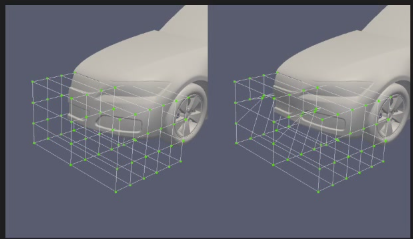
\includegraphics[width=0.309\textwidth]{pic/ACG6/FFD.png}
        \caption{FFD}
    \end{figure}
    \item Multi-resolution editing (多分辨率编辑)
    \begin{figure}[!htb]
        \centering
        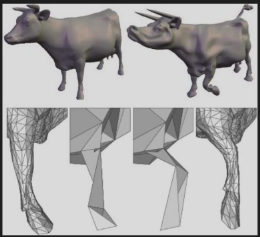
\includegraphics[width=0.309\textwidth]{pic/ACG6/Multi-resolution editing}
        \caption{Multi-resolution editing}
    \end{figure}
    \item Differential domain methods (微分域方法)
\end{itemize}

\subsection{Differential domain methods}
(做研究首先要确定目标)

\subsubsection{Goal}
\begin{itemize}
    \item High quality: smooth deformation, detail preservation 
    \item Easy manipulation: anchor-based, sketch-based
    \item Useful constraints: volume, skeleton, projection, ...
    \item Popular inputs: subdivsion, skinned mesh, man-made
    \item Interactive speed: nonlinear, optimization, GPU
\end{itemize}

\subsubsection{Detail preservation}
Detail: 

gradients:
\begin{align*}
    \nabla F&=\left( \pard{F}{x}, \pard{F}{y}, \pard{F}{z} \right)\\
    \nabla F&= F_1 \psi_1 + F_2 \psi_2 + F_3 \psi_3
\end{align*}

\begin{figure}[!htb]
    \centering
    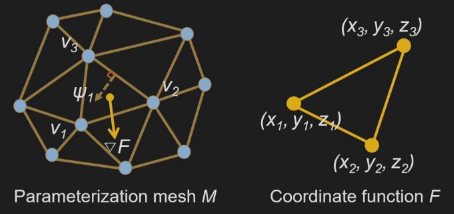
\includegraphics[width=0.309\textwidth]{pic/ACG6/Detail}
    \caption{gradients}
\end{figure}

Manipulate gradients:
\begin{align*}
    G&= F'_1 \psi_1 + F'_2 \psi_2 + F'_3 \psi_3\\
    &\min_F \int_M \norm{\nabla F-G}^2
\end{align*}

\begin{figure}[!htb]
    \centering
    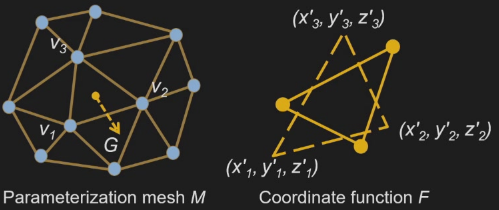
\includegraphics[width=0.309\textwidth]{pic/ACG6/Manipulate gradients}
    \caption{Manipulate gradients}
\end{figure}

Poisson equation:
\begin{align*}
    \Delta F &= \mathrm{div} G \text{ with }F|_\Omega = F^*|_\Omega\\
    \Delta F(v_i)&=v_i-\sum_{j=1}^{n_i}w_{ij}v_{i,j}\\
    \mathrm{div} G(v_i)&=\sum_{t_k\in N(v_i)}\rho_{ki}\cdot G(t_k)|t_k|\\
    AF&=b
\end{align*}
$\Delta$ is Laplacian, $\mathrm{div}$ is Divergence.

\begin{figure}[!htb]
    \centering
    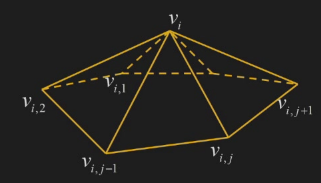
\includegraphics[width=0.22\textwidth]{pic/ACG6/Poisson equation}
    \caption{Poisson equation}
\end{figure}

Poisson mesh editing:
\begin{itemize}
    \item Sommthly changing gradients: 因为从梯度到坐标点, 可以保证坐标变换的光滑
    \item Global optimization: 平均分布的误差
\end{itemize}

\begin{figure}[!htb]
    \centering
    \begin{subfigure}{0.22\textwidth}
        \centering
        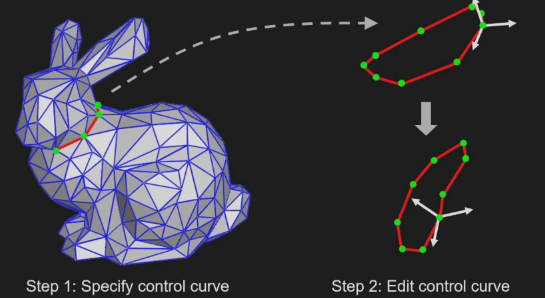
\includegraphics[height=0.54\textwidth]{pic/ACG6/Poisson mesh editing1.png}
        % \caption{}
    \end{subfigure}
    \begin{subfigure}{0.22\textwidth}
        \centering
        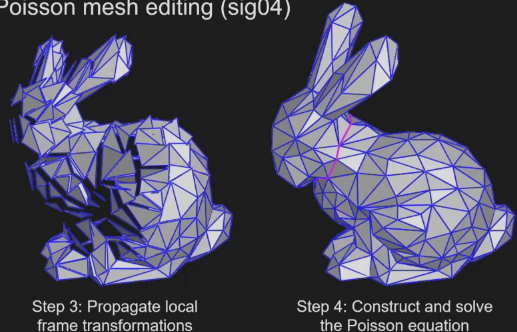
\includegraphics[height=0.54\textwidth]{pic/ACG6/Poisson mesh editing2.png}
        % \caption{}
    \end{subfigure}
    \caption{Poisson mesh editing}
\end{figure}

Laplacian surface editing:
\begin{align*}
    \delta_i&=L(v_i)=v_i-\sum_{j=1}^{n_i}w_{ij}v_{i,j}\\
    L(v_i)&=\delta_i\\
    AV&=b
\end{align*}

Preserving surface details is not enough: Bending and Twisting

已经昏了, 不想记了, 开摆!

非线性能量函数优化:
\begin{enumerate}
    \item 子空间: 在在空间求解
    \item 分段迭代: 先迭代易收敛的, 再以其为初始值迭代其他的
    \item 瀑布求解: 先加基本约束, 再逐渐加其他约束.
\end{enumerate}